%\documentclass{article}
%\usepackage{blindtext}
%\usepackage[a4paper, total={6in, 9.4in}]{geometry}

\documentclass[a4paper, 12pt]{article}

\usepackage[english, russian]{babel}
\usepackage[T2A]{fontenc}
\usepackage[utf8]{inputenc}
\usepackage{mathtext}
\usepackage{amsfonts}
\usepackage{ amssymb }
\usepackage{amsmath}
\usepackage{graphics}
\usepackage{graphicx}
\usepackage{wrapfig}
\usepackage{geometry}
\usepackage{float}
\geometry{
	a4paper,
	total={170mm, 257mm},
	left=20mm,
	top=10mm}
	
\usepackage{wrapfig}
\usepackage{graphicx}
\usepackage{mathtext}
\usepackage{amsmath}
\usepackage{siunitx} % Required for alignment
\usepackage{subfigure}
\usepackage{multirow}
\usepackage{rotating}
\usepackage{afterpage}
\usepackage[T1,T2A]{fontenc}
\usepackage[russian]{babel}
\usepackage{caption}
\usepackage[arrowdel]{physics}
\usepackage{booktabs}
\usepackage{float}

\graphicspath{{pictures/}}

\title{\begin{center}Лабораторная работа №3.7.1\end{center}
	Скин-эффект в полом цилиндре}
\author{Абакшин Василий, Б05-207}
\date{\today}

\begin{document}
	\maketitle
	\textbf{Цель работы:} Исследование проникновения переменного магнитного поля в медный полый цилиндр
	
	\section*{Теоретическая часть}
	\subsection*{Скин-эффект для полупрастранства}
	\vspace{1cm}
	\begin{wrapfigure}{l}{0.3\textwidth}
		\begin{center}
			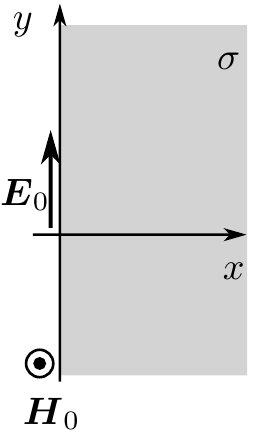
\includegraphics[width=0.28\textwidth]{poluprostranstvo}
		\end{center}
		%\caption{Скин-эффект в полупространстве}\label{fig:poluprostranstvo}
	\end{wrapfigure}
	
	Рассмотрим квазистационарное поле внутри проводящей среды в простейшем плоском случае.
	Пусть вектор $\vb*{E}$ направлен всюду вдоль оси $y$ и зависит только от координаты $x$, т. е. ${E_x} = {E_z} \equiv 0$, $E_y=E_y(x,t)$.
	В квазистационарном приближении 
	\begin{equation*}
		\grad \times \vb*{H} = \sigma \vb*{E}
	\end{equation*}
	
	Преобразуя это уравнение, можно получить уравнение, схожее с уравнением диффузии:
	\begin{equation}
		\grad^2\vb*{H}=\sigma\mu\mu_0 \frac{\partial \vb*{H}}{\partial t}\label{eq:laplacian_H}
	\end{equation}
	Точно такое же уравнение имеет место и для вектора $E:$
	\begin{equation}
		\grad^2\vb*{E}=\sigma\mu\mu_0 \frac{\partial \vb*{E}}{\partial t}\label{eq:diffusion}
	\end{equation}
	
	Подставляем в (\ref{eq:diffusion}) наше электрическое поле $E_y=E_y(x,t)$
	\begin{equation}
		\frac{\partial^2 E_y}{\partial x^2} = \sigma\mu\mu_0\frac{\partial E_y}{\partial t}
		\label{eq:diffusion_chastni}
	\end{equation}
	Если $E_y(0,t)=E_0 e^{i\omega t}$ то решением (\ref{eq:diffusion_chastni}) будет функция вида
	\begin{equation}
		E_y(x,t)=E_0 e^{-x/\delta} e^{i(\omega t - x/\delta)}
		\label{eq:skin_effect_poluprostranstvo}
	\end{equation}
	где
	\begin{equation}
		\delta = \sqrt{\frac{2}{\omega\sigma\mu\mu_0}}
		\label{eq:delta}
	\end{equation}
	
	\newpage
	\subsection*{Скин-эффект в тонокм полом цилиндре}
	\vspace{1cm}
	\begin{wrapfigure}[36]{l}{0.3\textwidth}
		\begin{center}
			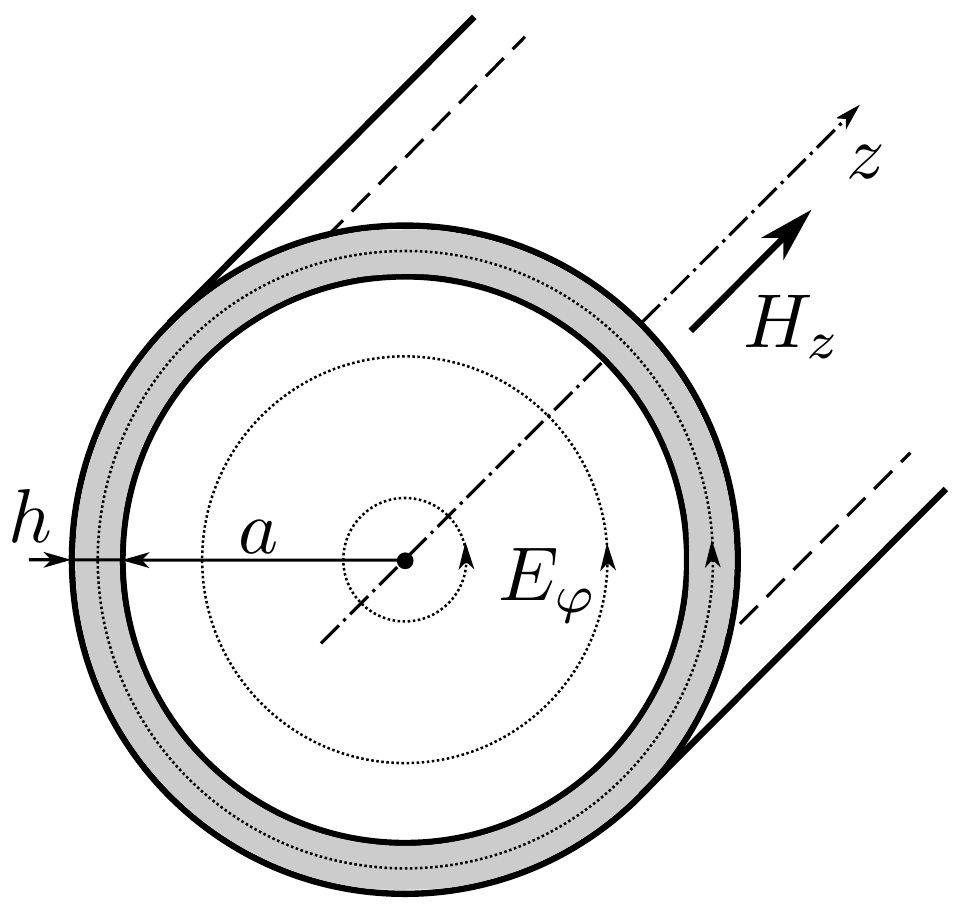
\includegraphics[width=0.28\textwidth]{cilindr}
		\end{center}
		\caption{Эл-магнитные поля в цилиндре}\label{fig:cilindr}
		
		\begin{center}
			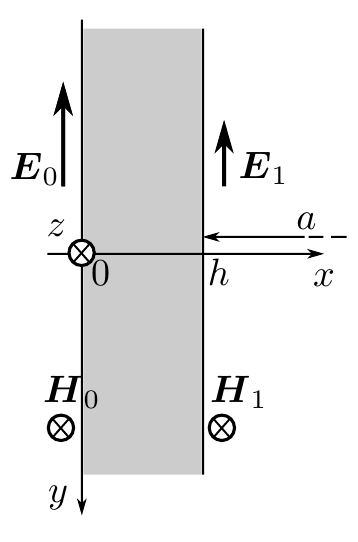
\includegraphics[width=0.28\textwidth]{stenka}
		\end{center}
		\caption{Стенка цилиндра}\label{fig:stenka}
	\end{wrapfigure}
	
	Перейдем теперь к описанию теории в нашей работе. Из соображении симметрии и 
	непрерывности соответствующих компонет векторов $\vb*{E}$ и $\vb*{H}$ можем сказать что
	\begin{equation*}
		H_z = H(r)e^{i\omega t} \text{, } E_\varphi = E(r)e^{i\omega t}
	\end{equation*}
	и при этом функции $H(r)$ и $E(r)$ непрерывны.
	
	Внутри цилиндра токов нет, следовательно $H(r)=H_1=\text{const}$ внутри цилиндра.
	По теореме об электромагнитной индукции
	\begin{equation*}
		E(r) = -\frac{1}{2}\mu_0 r \cdot i \omega H_1
	\end{equation*}
	откуда мы получаем граничное условие
	\begin{equation}
		E_1=E(a)= -\frac{1}{2}\mu_0 a \cdot i \omega H_1
		\label{eq:granichnoe_uslovie_E}
	\end{equation}
	
	В прближении $h \ll a$ можем пренебречь кривизной стенки и смоделировать 
	его бесконечной полосой. Тогда, надо решить уравнение (\ref{eq:laplacian_H})
	с граничными условиями. Решая уравнение получим связь полей $H_1$ 
	(поле внутри цилиндра которое мы будем измерять) и $H_0$, которое колебается с частотой
	$\omega$
	
	\begin{equation}
		H_1 = \frac{H_0}{\ch(\alpha h) + \frac{1}{2} \alpha a \sh(\alpha h)} 
		\text{\ \ \ }
		\alpha = \sqrt{i\omega \sigma \mu_0} = \frac{\sqrt{2}}{\delta}e^{i\pi/4}
		\label{eq:svyaz_poley}
	\end{equation}
	
	из этой формулы получим сколько по фазе отстает поле $H_1$ от $H_0$. При $\delta \ll h$
	(высокачастотная область)
	
	\begin{equation}
		\psi \approx \frac{\pi}{4} + \frac{h}{\delta} = 
		\frac{\pi}{4} + h \sqrt{\frac{\omega \sigma \mu_0}{2}}
		\label{eq:faza_high_freq}
	\end{equation}
	
	При $\delta \gg h$ (низкочастотная область)
	
	\begin{equation}
		\tg \psi \approx \frac{ah}{\delta^2} = \pi a h \sigma \mu \mu_0 \nu
		\label{eq:faza_low_freq}
	\end{equation}
	
	\subsection*{Установка и процесс измерения}
	\begin{wrapfigure}{l}{0.4\textwidth}
		\begin{center}
			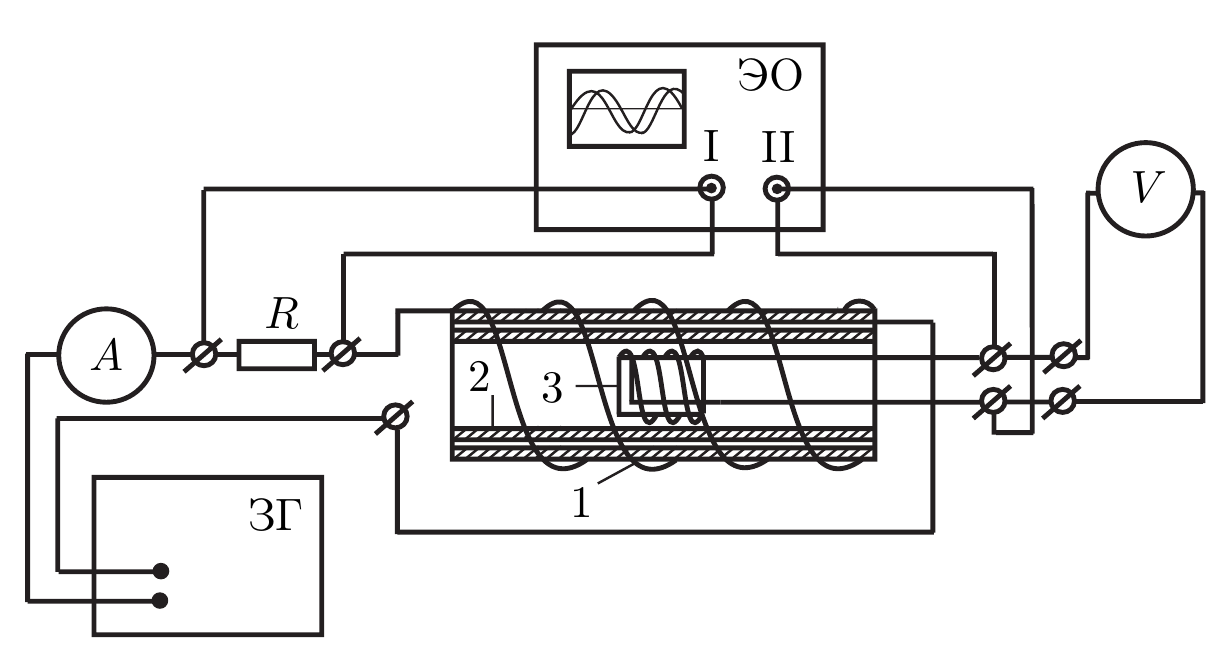
\includegraphics[width=0.38\textwidth]{ustanovka}
		\end{center}
		\caption{Установка}\label{fig:ustanovka}
	\end{wrapfigure}
	
	Переменное магнитное поле создается соленоидом 1, на который подается переменный ток со звукового генератора ЗГ. Внутри соленоида расположен медный экран 2. Магнитное поле внутри цилиндра измеряется катушкой 3. Напряжение на катушке пропорциональна производной $\dot{B_1}(t)$
	\begin{equation*}
		U(t) \propto \dot{B_1}(t) = -i\omega H_1 e^{i\omega t}
	\end{equation*}
	Поле внутри цилиндра пропорциональна току через соленоид
	\begin{equation*}
		H_0(t) \propto I(t)
	\end{equation*}
	Отсюда несложно увидеть, что
	\begin{equation}
		\frac{\abs{H_1}}{\abs{H_0}} = c \cdot \frac{U}{\nu I} = \xi_0 \xi
		\label{eq:otnoshenie_amplitud}
	\end{equation}
	где константу  $\xi_0$ можно определить из условия $\abs{H_1}/\abs{H_0} \rightarrow 1$ при
	$\nu \rightarrow 0$.\\
	
	При измерениях разности фаз нужно учесть, что первый сигнал на осциллографе
	пропорционален магнитному полю снаружи, а второй пропорционален производному
	поля внутри цилиндра по времени, поэтому измеренная на осциллографе разность фаз $\varphi$ будет на $\frac{\pi}{2}$ больше реальной $\psi$:
	\[\varphi = \psi + \frac{\pi}{2}\]

	\section*{Ход работы}
	
	Параметры нашей установки $2a = 45$ мм, $h=1.5$ мм. Проводимость порядка
	$\sigma \sim 5\cdot 10^7$ См/м. Получаем оценку для частоты, при которой
	глубина проникновения равна толщине стенок цилиндра $\nu_h = 2254$ Гц.
	
	\subsection*{Измерения амплитуд в области низких частот}
	В области низких частот толщина скин-слоя превосходит толщину образца $ \delta \gg h$  и из (\ref{eq:svyaz_poley}) получаем
	\begin{equation*}
		\left(\frac{|H_1|}{|H_0|}\right)^2 = (\xi_0\xi)^2 \approx \frac{1}{1+\left(\frac{ah}{\delta^2}\right)^2} = \frac{1}{1 + \left(\pi ah\nu\mu_0\sigma\right)^2}
	\end{equation*}
	Тогда: 
	\begin{equation*}
		\frac{1}{\xi^2}=\xi_0^2B^2\nu^2 + \xi_0^2 \text{, где } B=\pi a h \sigma \mu_0
		\label{eq:liniya_dlya_c}
	\end{equation*}
	\begin{figure}[h!]
		\centering
		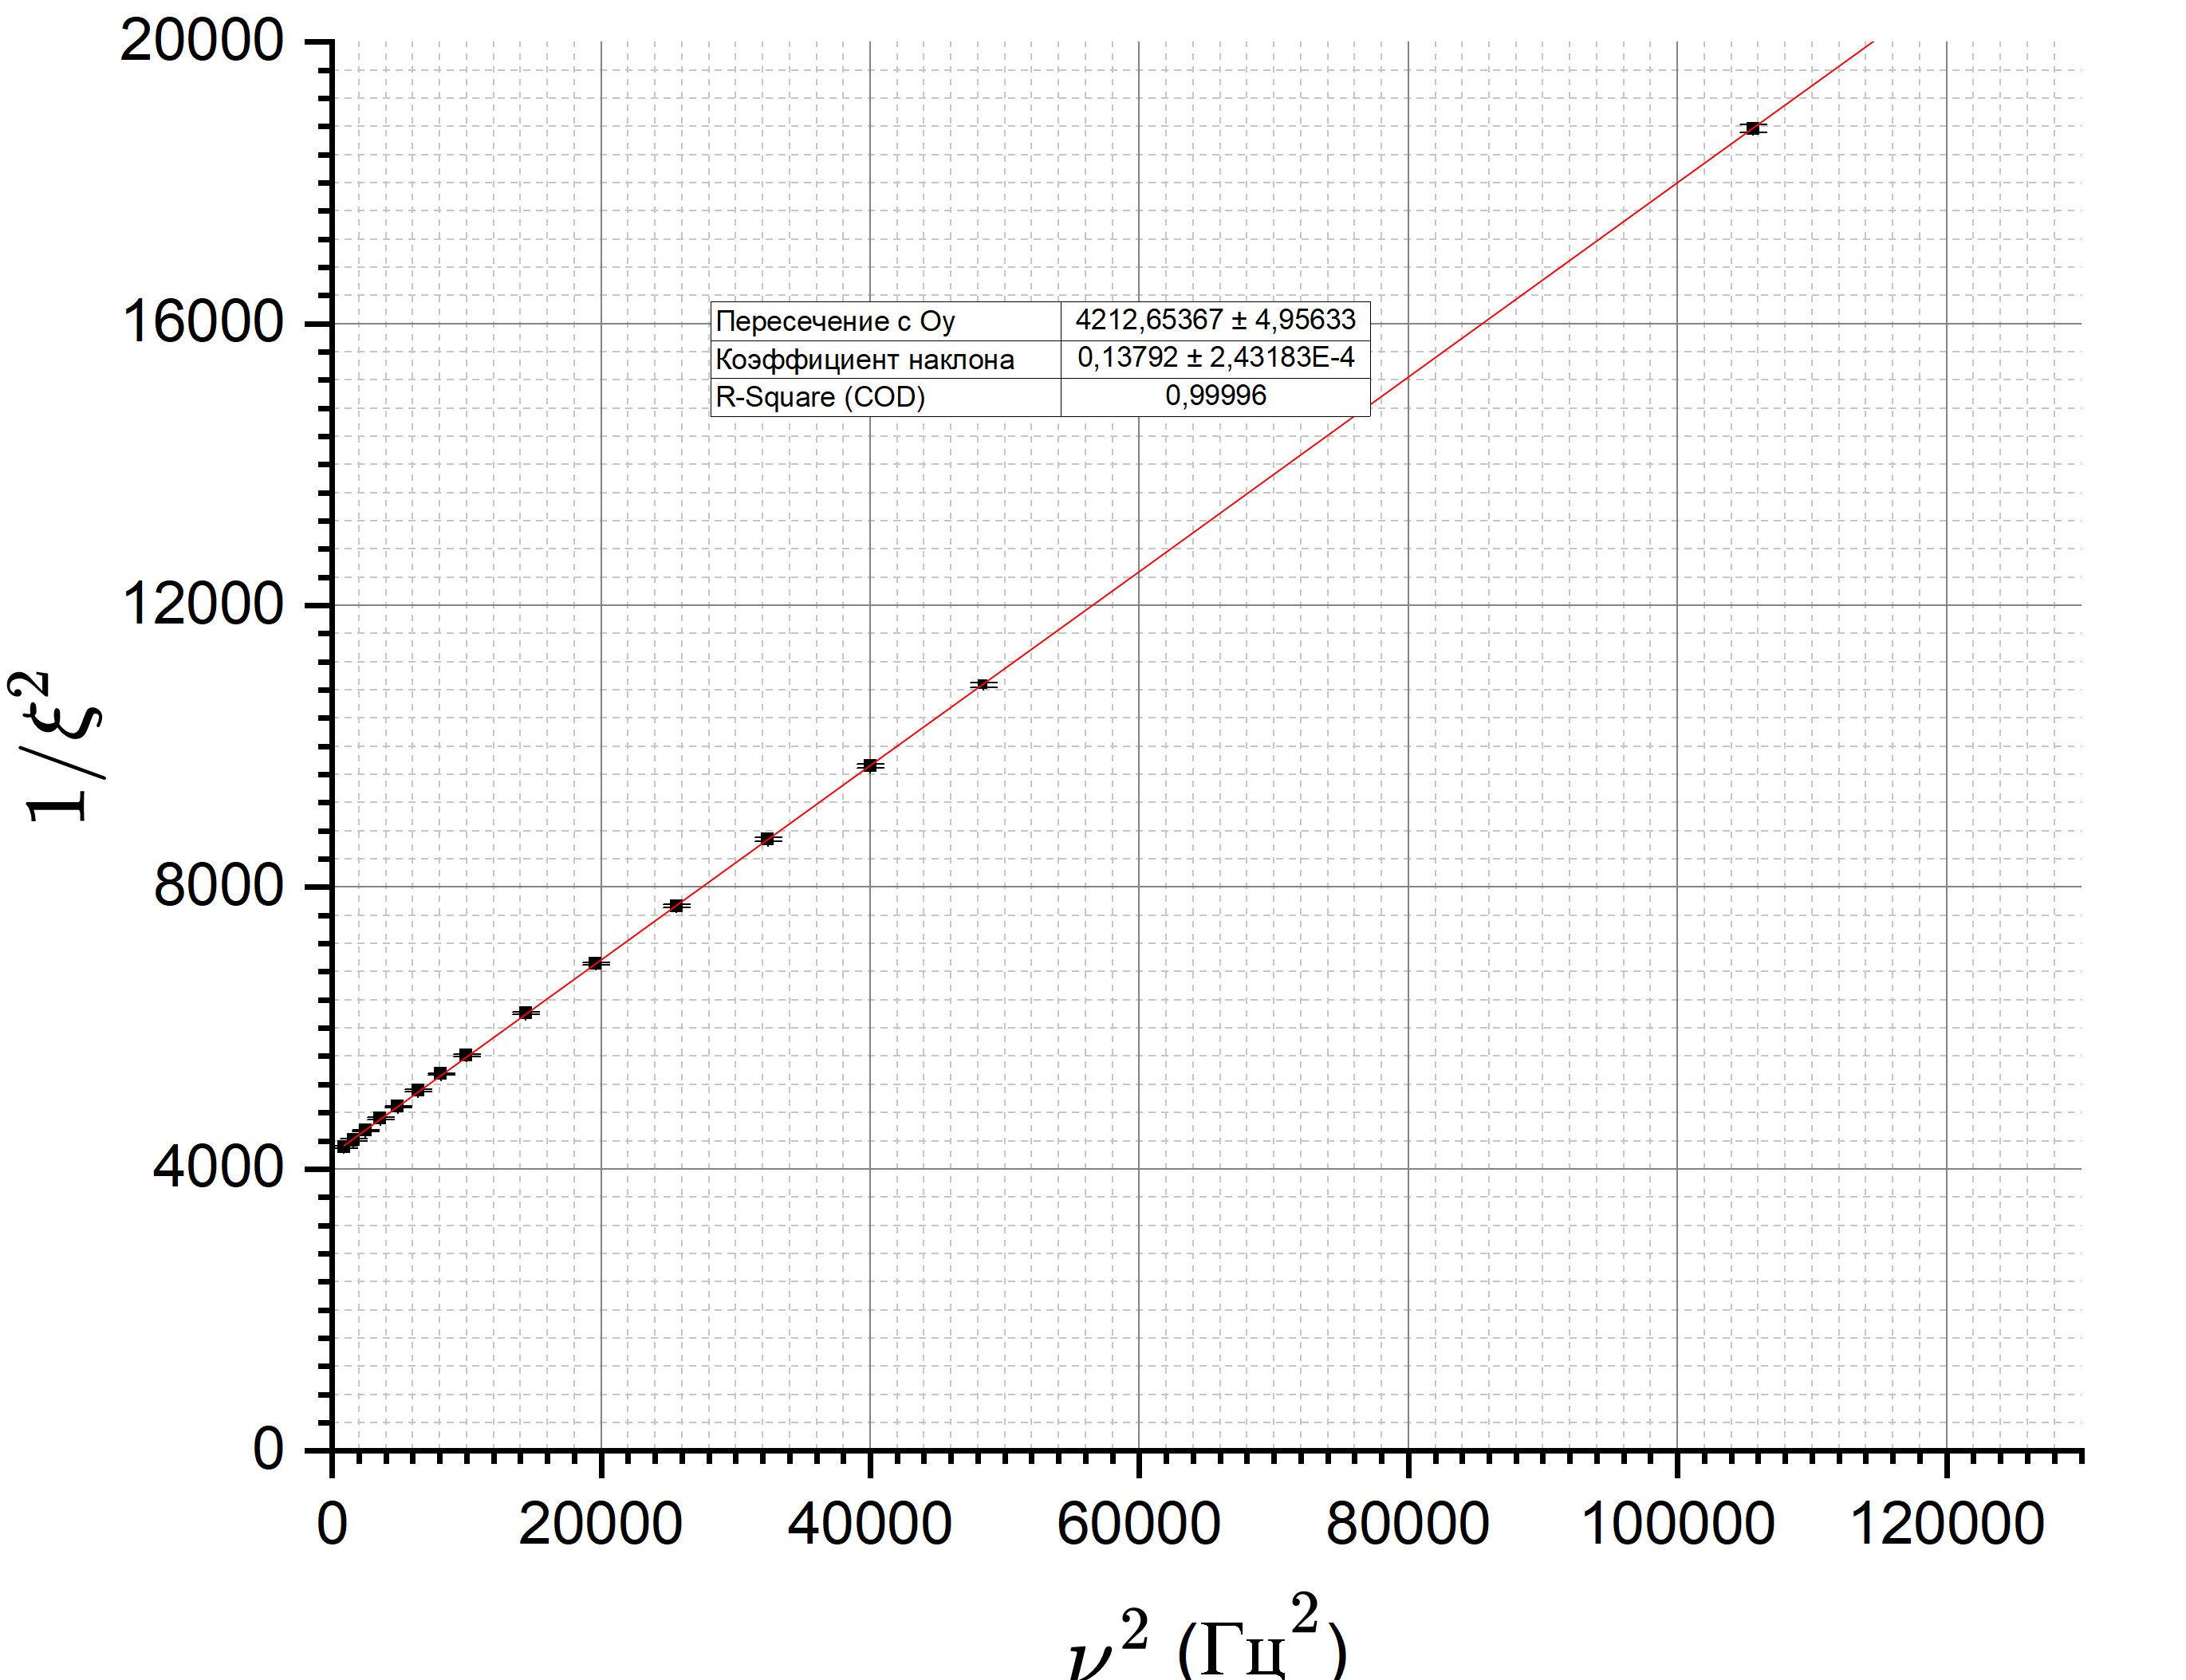
\includegraphics[width=0.9\textwidth, height = 0.45\textheight]{Low_Freq}
		\caption{График зависимости $1/\xi^2(\nu^2)$}\label{fig:xi_nu_low_freq_linearized}
	\end{figure}
	Получаем следующие значения: $\xi_0^2B^2 = 0.138, \ \xi_0^2 = 4212.65$, тогда:
	\[\xi_0 = 64.90 \pm 0.04 \ \frac{\text{Гц}}{\text{Ом}}, \ \sigma = (4.294 \pm 0.005) \cdot 10^7 \ \frac{\text{См}}{\text{м}}  \]
	
	\subsection*{Измерение проводимости через разность фаз при низких частотах}
	Построим график $\tg{\psi} (\nu)$ по тем точкам точкам, для которых он хорошо аппроксимируется прямой (при $\nu \approx 0.5 \nu_h \ \tg \psi \rightarrow +\infty$) 
	Согласно формуле (\ref{eq:faza_low_freq}), при $\delta \gg h$
	\begin{equation*}
		\tg \psi = \frac{ahw \sigma \mu_0}{2} = \pi ah\mu_0\sigma \nu \ \ (\mu = 1)
	\end{equation*}
	Коэффициент наклона прямой: \[\pi ah \mu_0\sigma = k = (5.2 \pm 1) \cdot 10^{-3} \ \text{с}\]
	\[\sigma = \frac{k}{\pi ah \mu_0} = (3.93 \pm 0.73) \cdot 10^7 \ \frac{\text{См}}{\text{м}}\]
	\begin{figure}[H]
		\centering
		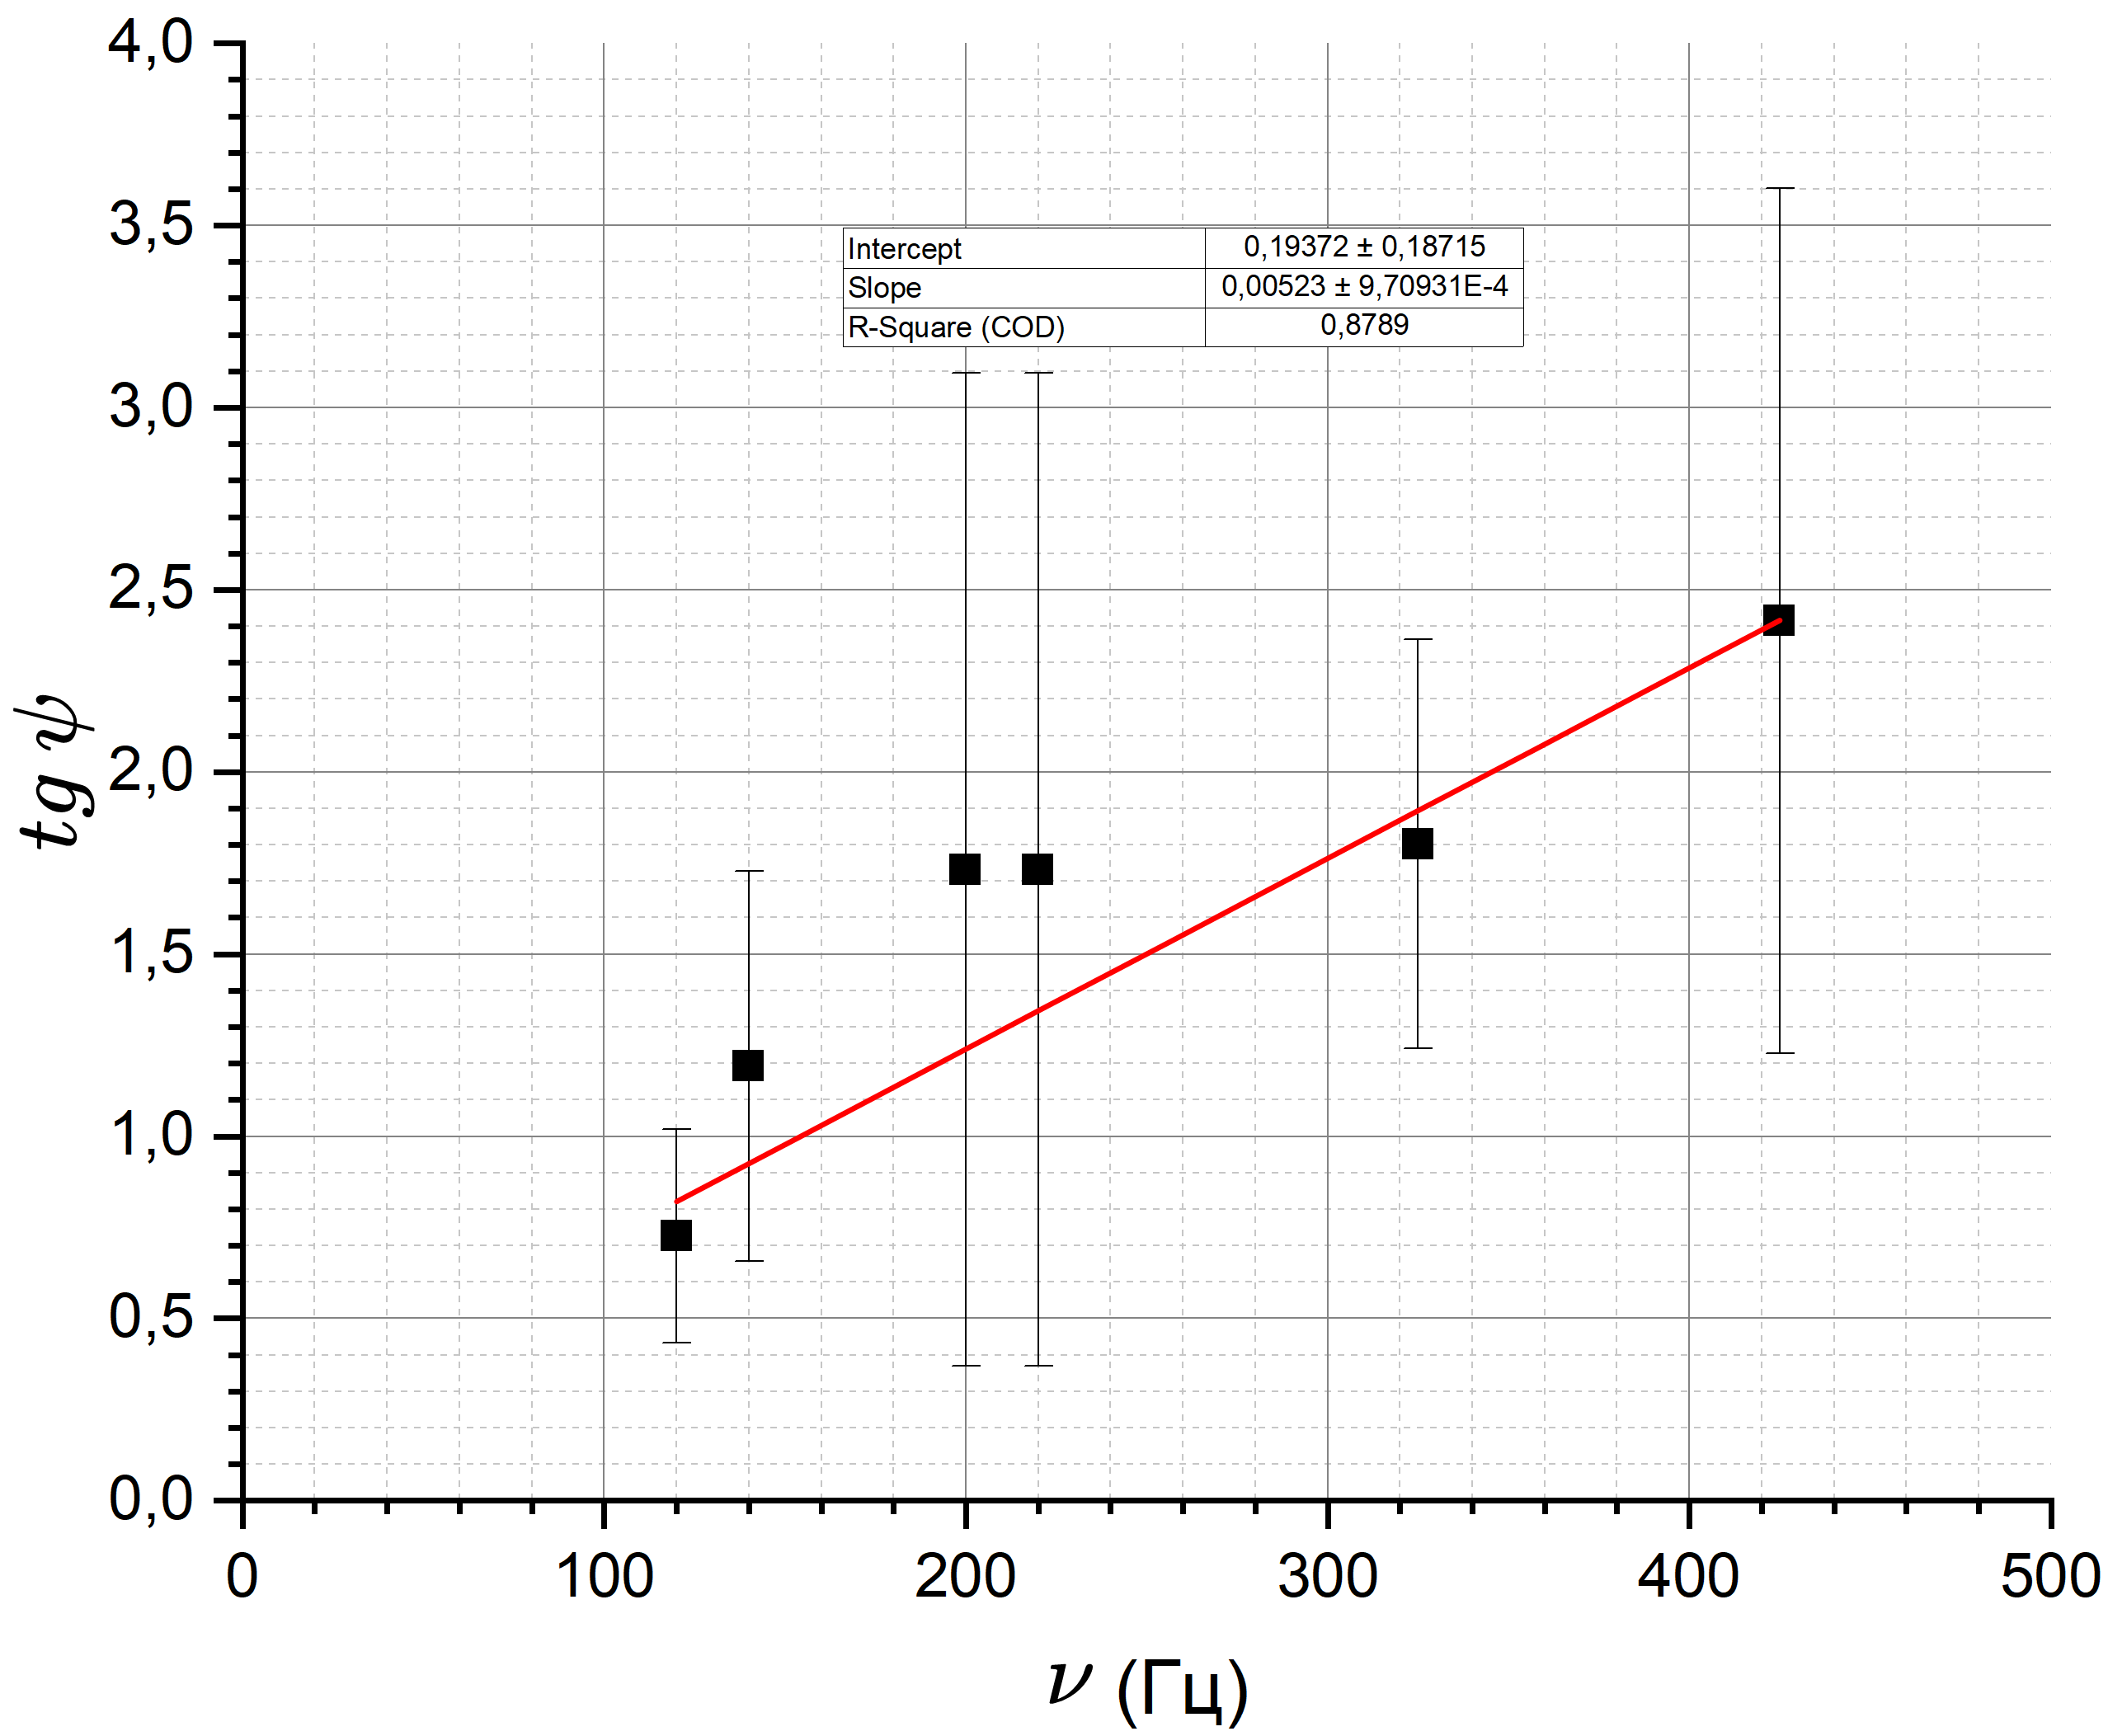
\includegraphics[width=0.9\textwidth, height = 0.45\textheight]{Phase_diff_1}
		\caption{График зависимости $\tg \psi (\nu)$}\label{fig:tg_psi_nu_line}
	\end{figure}

	\subsection*{Измерение проводимости через разность фаз в высокочастотном диапазоне}
	Согласно формуле (\ref{eq:faza_high_freq}), при $\delta \ll h$
	\begin{equation*}
		\psi - \pi/4 = k\cdot \sqrt{\nu}; \ k = h\sqrt{\pi\mu_0\sigma}
	\end{equation*}
	
	Получено значение $k = 0.0184 \pm 0.0014$, отсюда получаем значение проводимости:
	
	\begin{equation}
		\sigma = (3.80 \pm 0.58) \cdot 10^7 \ \frac{\text{См}}{\text{м}}
	\end{equation}
	
	\begin{figure}[h]
		\centering
		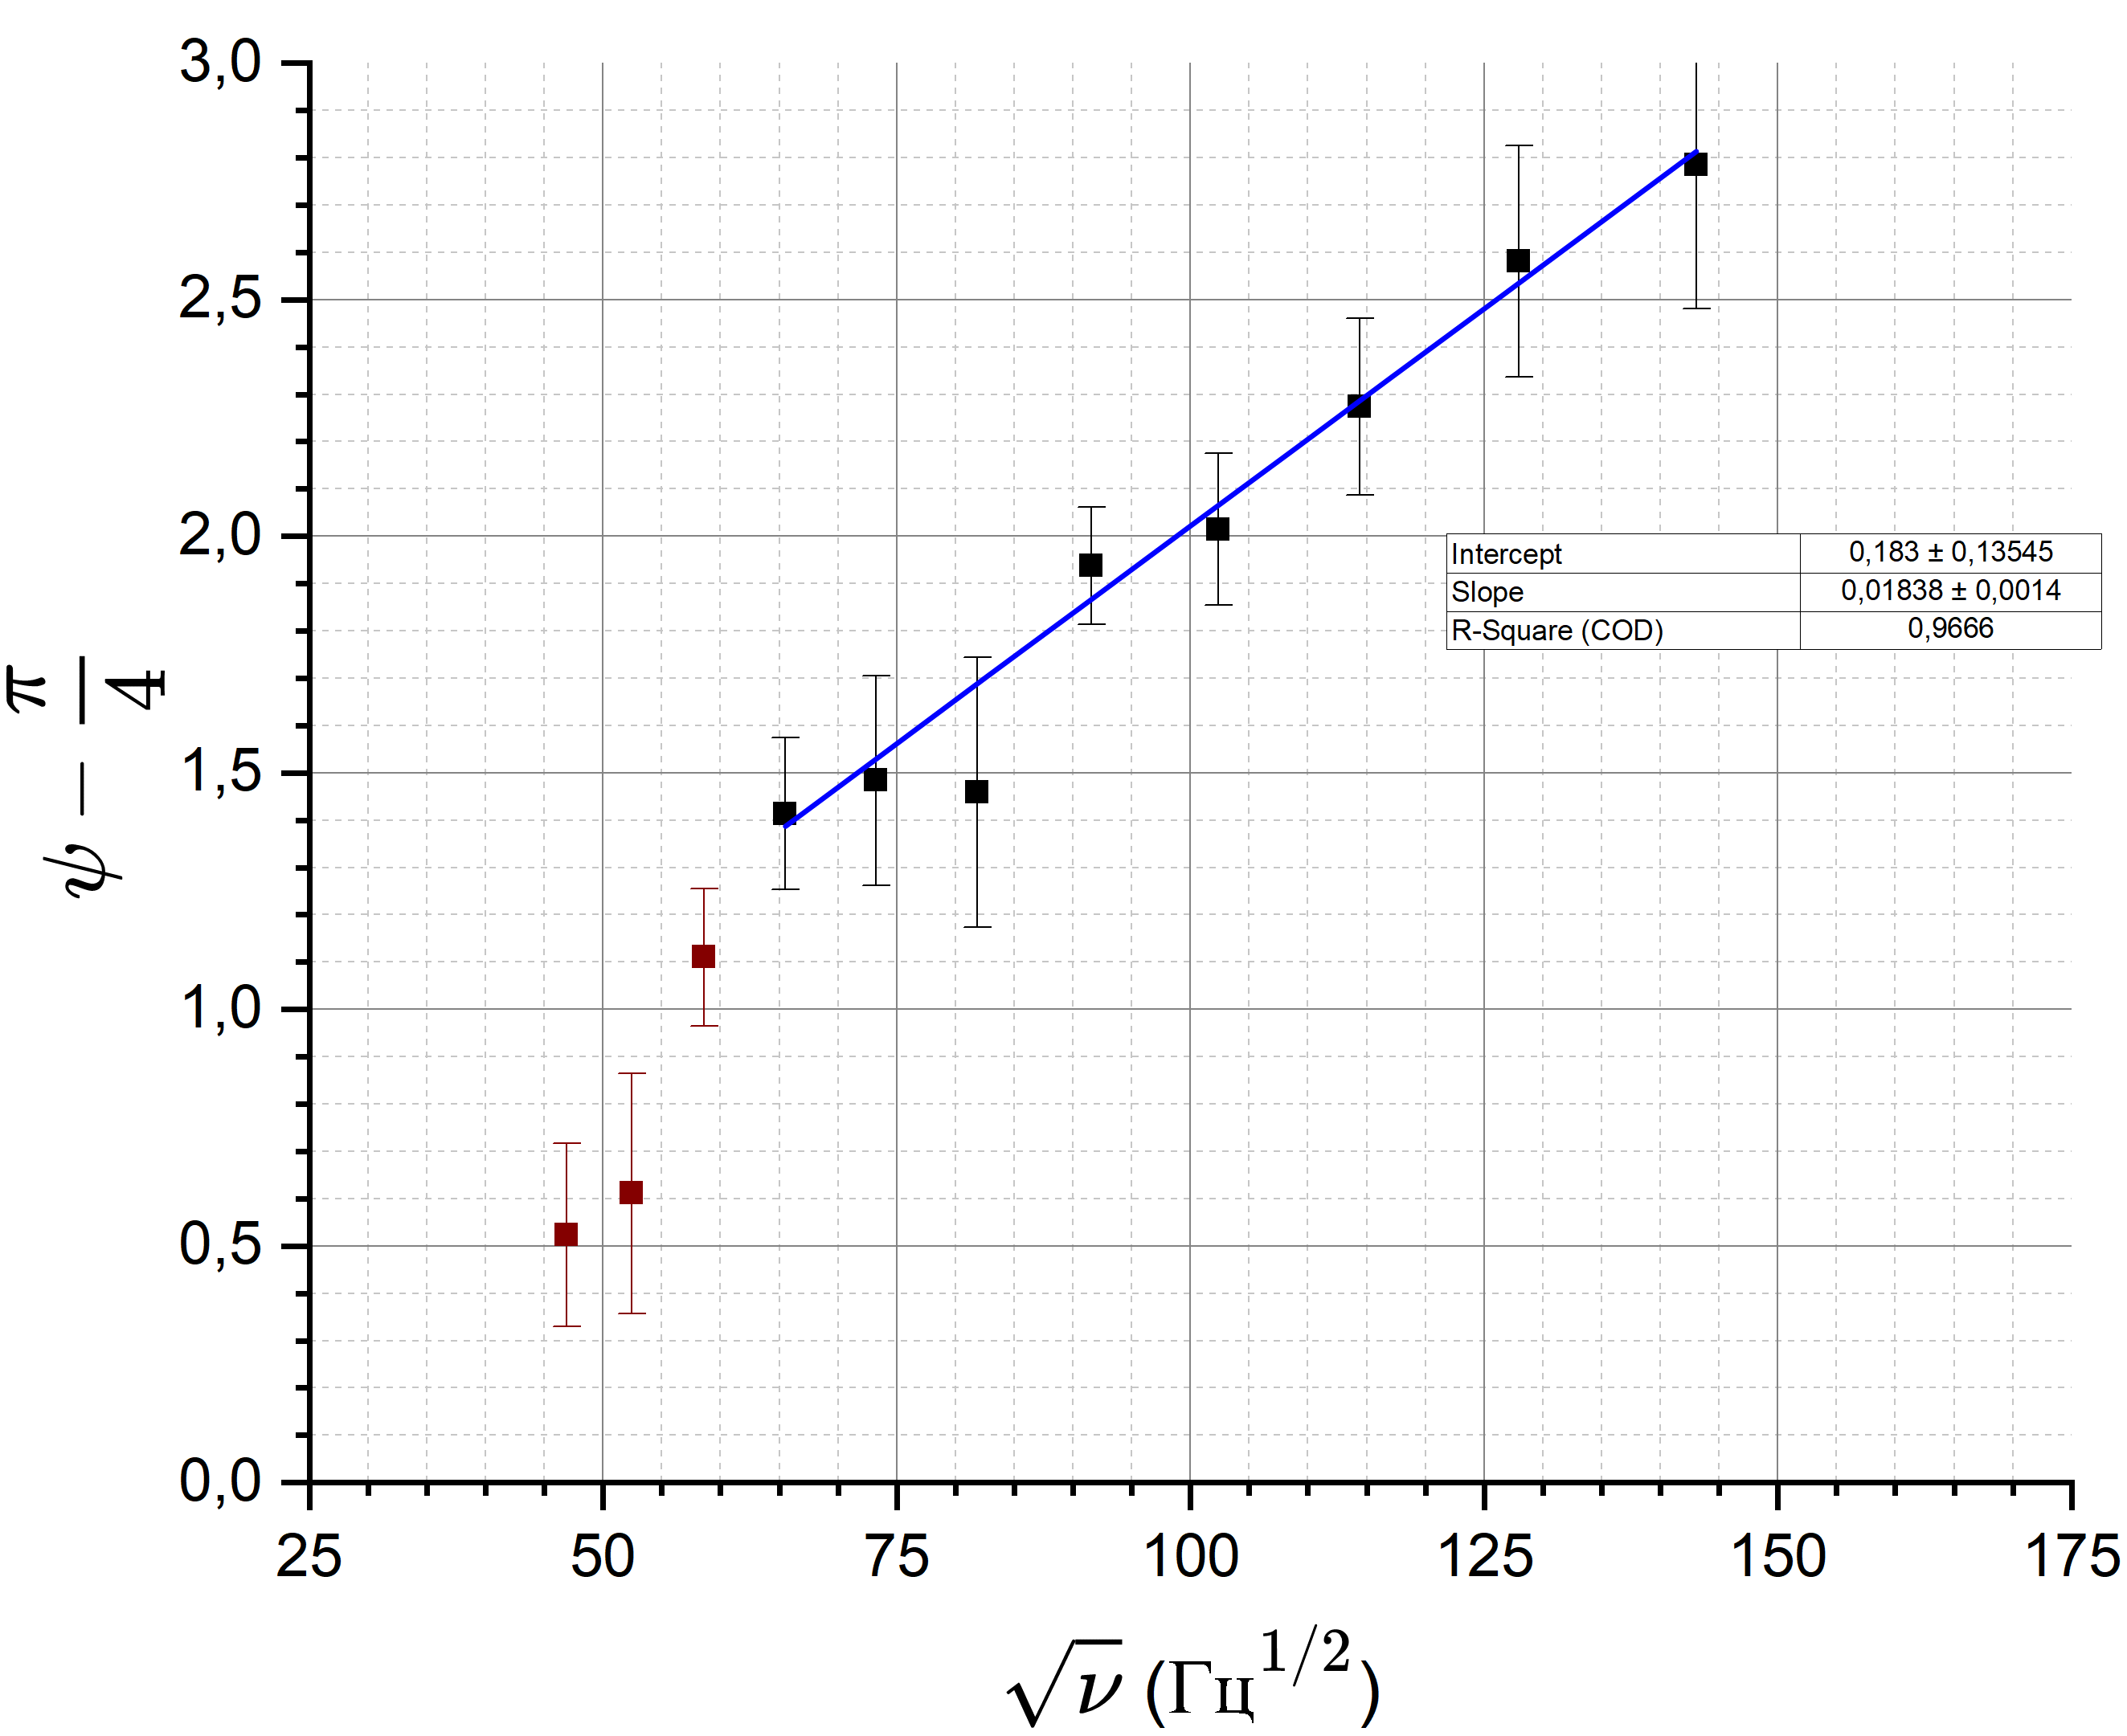
\includegraphics[width=\textwidth]{High_freq}
		\caption{График зависимости $(\psi - \pi/4)(\sqrt{\nu})$}
		\newpage
	\end{figure}
	
	\subsection*{Измерение проводимости через изменение индуктивности}
	Измерить проводимость можно также через изменение индуктивности катушки внутри цилиндра. Данные, измеренные с помощью $RCL$-метра:
	
	\begin{table}[h!]
		\centering
		\begin{tabular}{|c|c|c|c|c|c|c|c|c|c|c|c|c|c|c|}
			\hline
			$\nu$, кГц & 0.04 & 0.15 & 0.25 & 0.3 & 0.4 & 0.5 & 0.6 & 0.8 & 1.5 & 2.5 & 4 & 10 & 15 & 20 \\
			\hline
			$L$, мГн & 10 & 7.35 & 5.4 & 4.8 & 4.0  & 3.65 & 3.45 & 3.26 & 2.9 & 2.9 & 2.9 & 3 & 3.17 & 3.6 \\
			\hline
		\end{tabular}
		\caption{Значения индуктивности катушки при различных частотах}
	\end{table}
	
	Примерно так выглядит график $L(\nu)$:
	
	\begin{figure}[H]
		\centering
		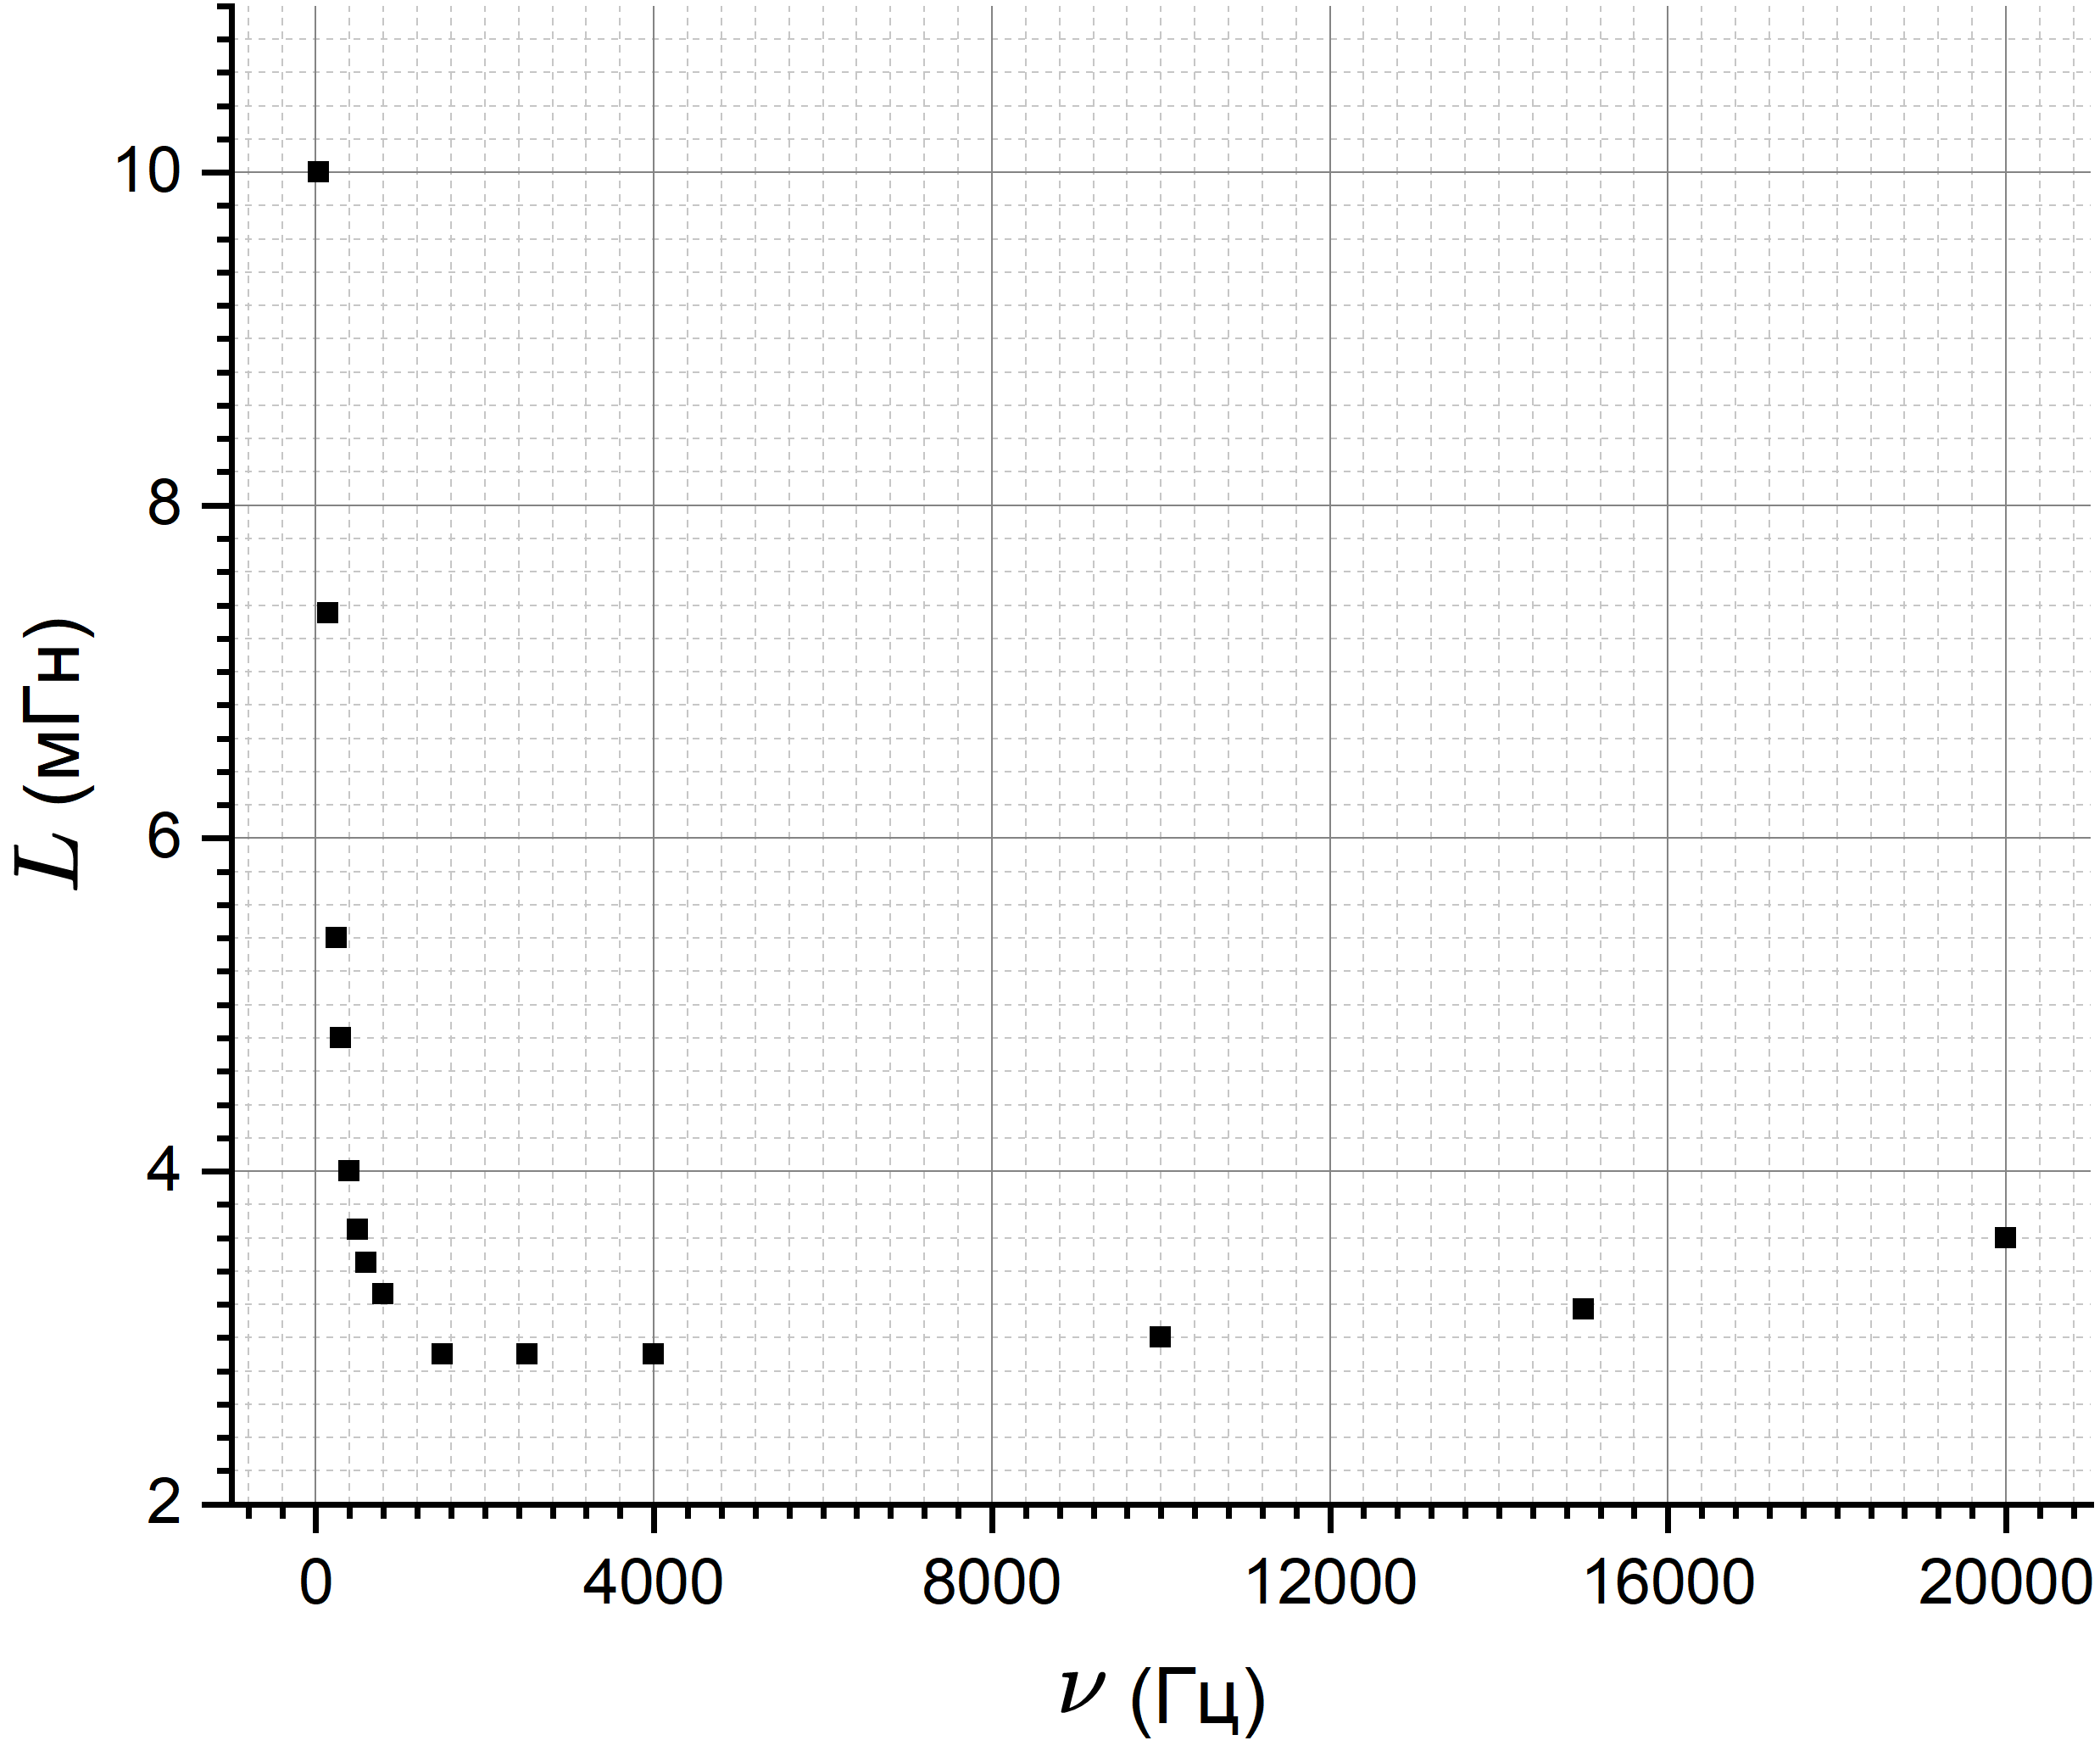
\includegraphics[width = \textwidth]{L(nu)}
		\caption{График зависимости $L(\nu)$}
	\end{figure}
	
	Полученные максимальные и минимальные значения: $L_{min} = 2.9$ мГн, $L_{max} = 10$ мГн.
	\begin{equation*}
		\frac{L_{\max} - L}{L - L_{\min}} = \pi ^2 a^2 h^2 {\mu_0}^2 \sigma^2 \nu^2
	\end{equation*}
	
	То есть коэффициент наклона графика
	\[k = (\pi ah\mu_0 \sigma)^2 \ \rightarrow \sigma = \frac{\sqrt{k}}{\pi ah \mu_0}\]
	
	Подставляя полученные значения, получаем:
	
	\begin{equation}
		\sigma = (4.11 \pm 0.07) \cdot 10^7  \ \frac{\text{См}}{\text{м}}
	\end{equation}
	
	\begin{figure}[h!]
		\centering
		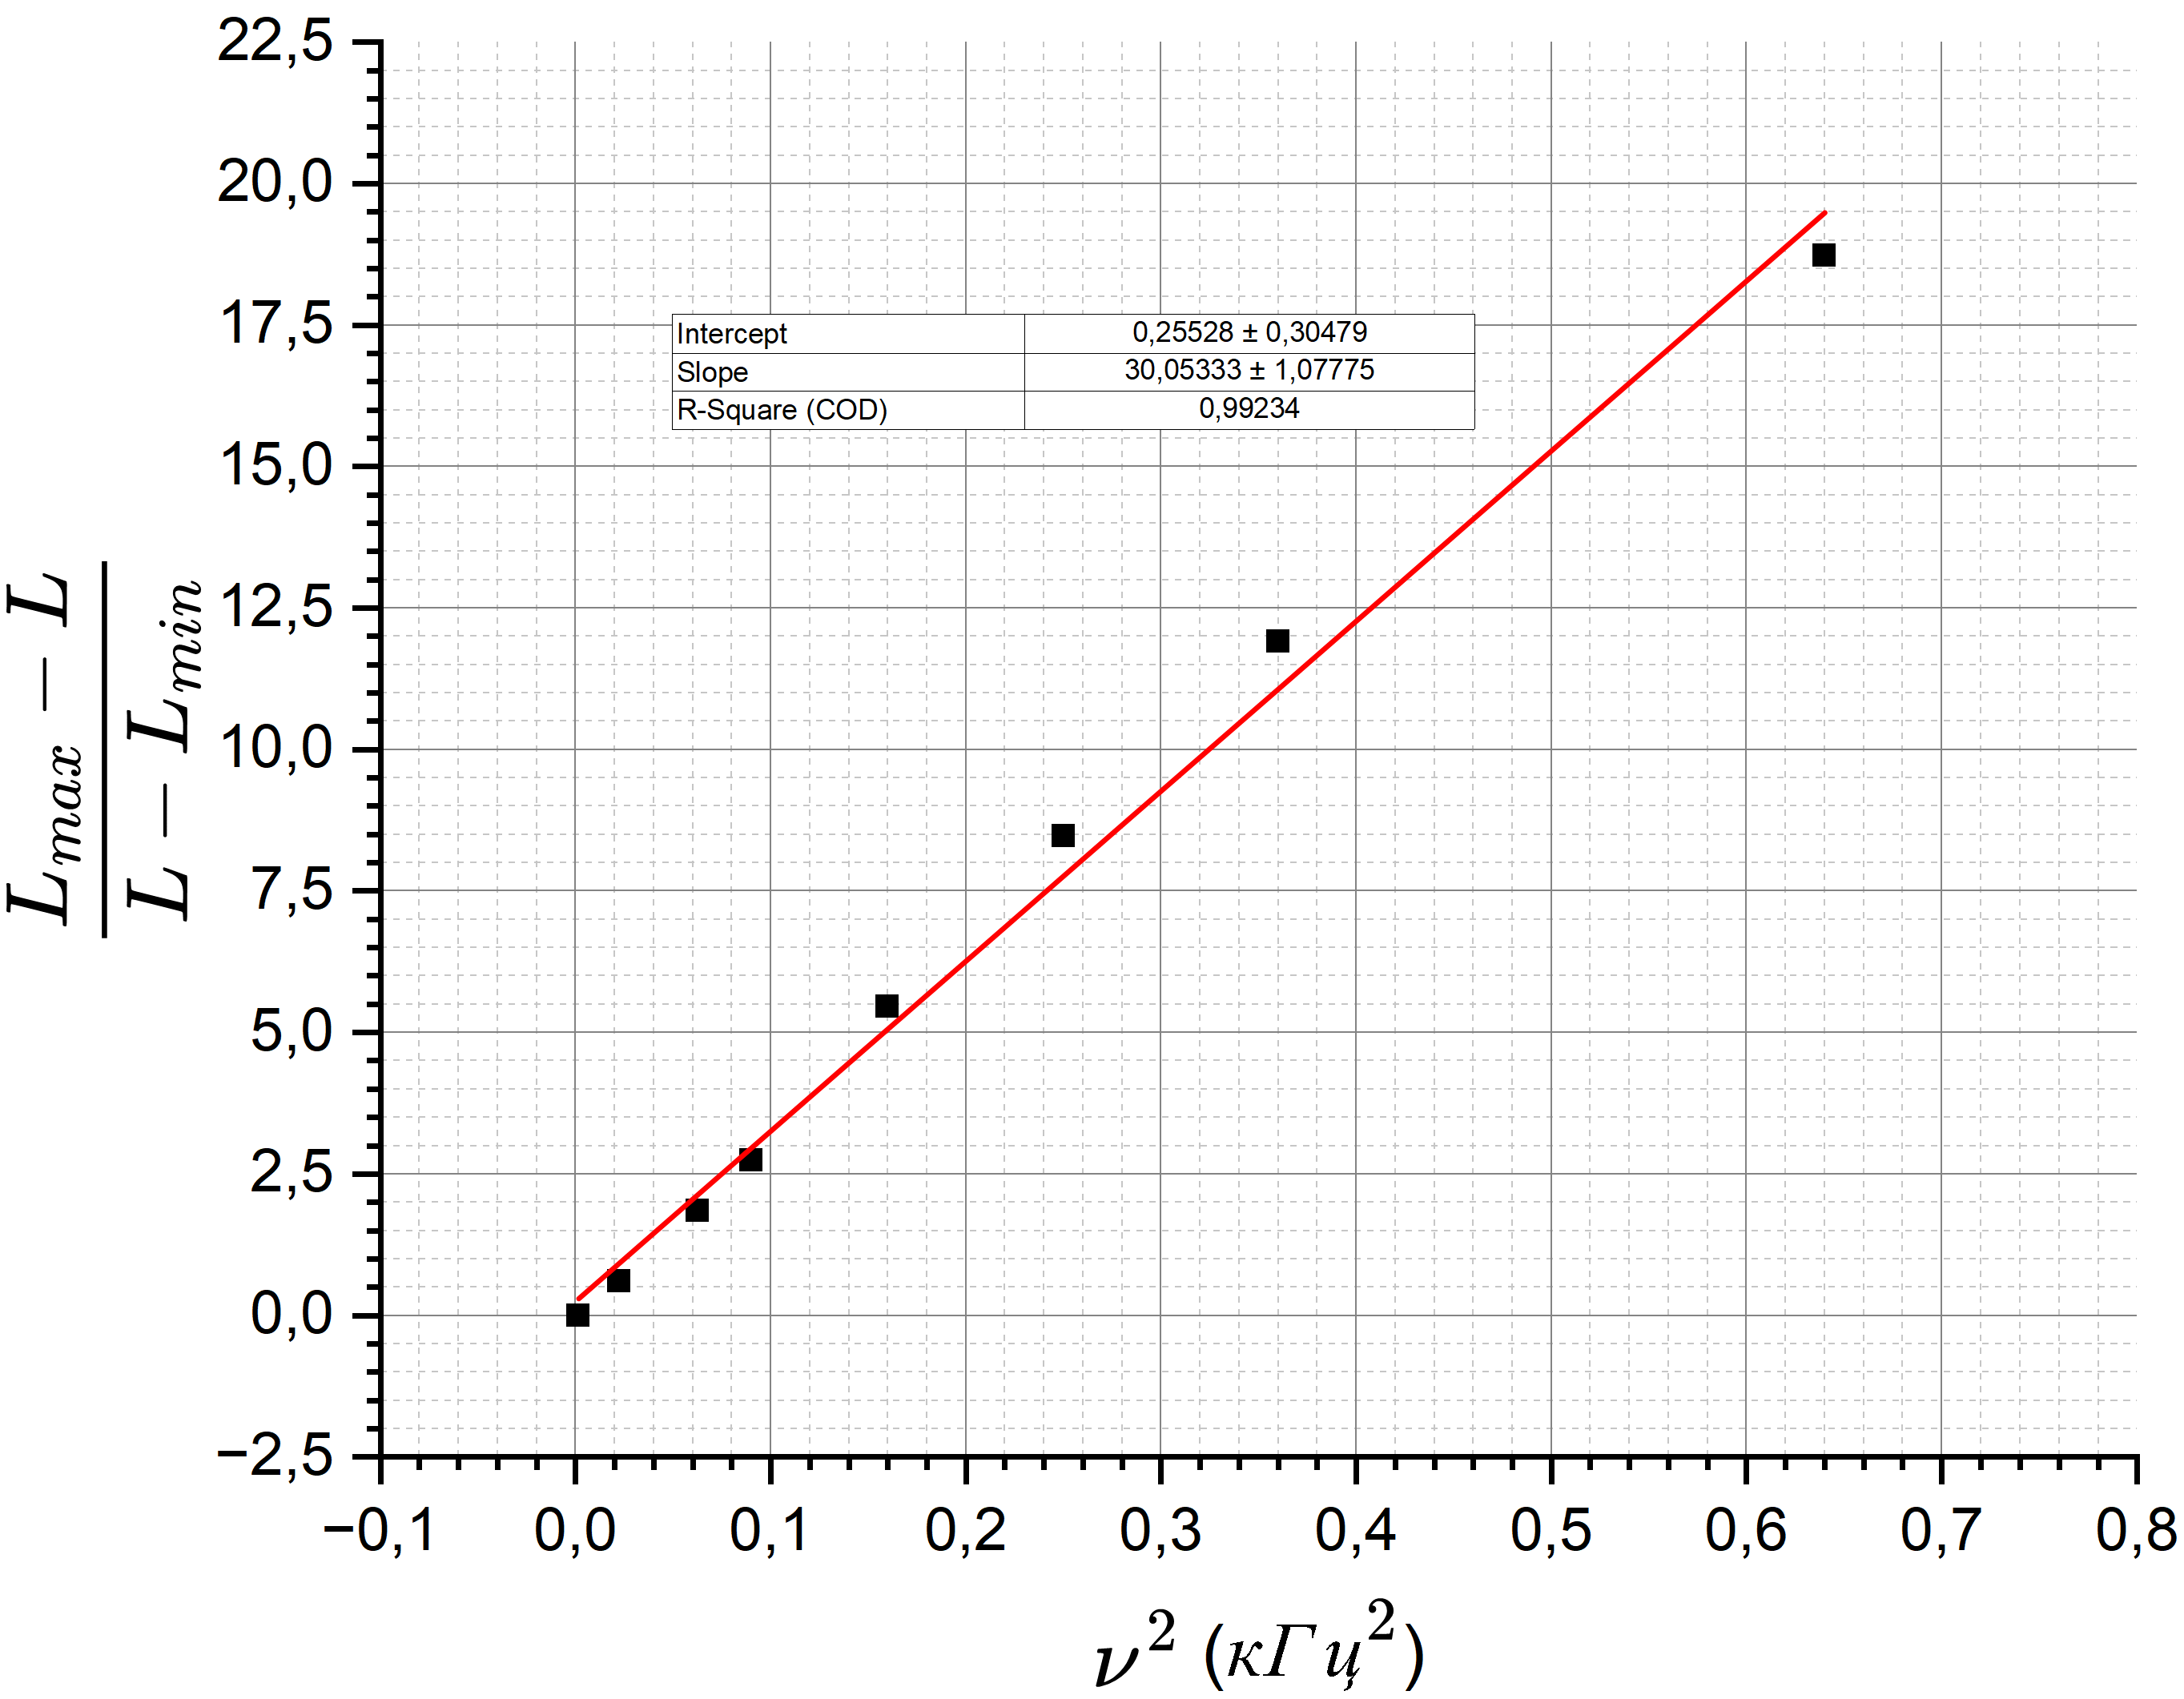
\includegraphics[width=\textwidth]{L_linear}
		\caption{График зависимости $\frac{L_{\max} - L}{L - L_{\min}} (\nu^2)$}
	\end{figure}
	
	
	\subsection*{Отношение магнитных полей}
	Отношение $\abs{H_1}/\abs{H_0}$ можем посчитать двумя способами. Первый способ - через
	формулу (\ref{eq:otnoshenie_amplitud}),использовав посчитанное значение $\xi_0$ в анализе амплитуд в области низких частот.
	Второй способ - через теоретическую формулу (\ref{eq:svyaz_poley}), использовав первое полученное значение $\sigma$. Посмотрим на их различие с помощью графиков зависимости
	$\abs{H_1}/\abs{H_0} (\nu)$
	
	\begin{figure}[h]
		\centering
		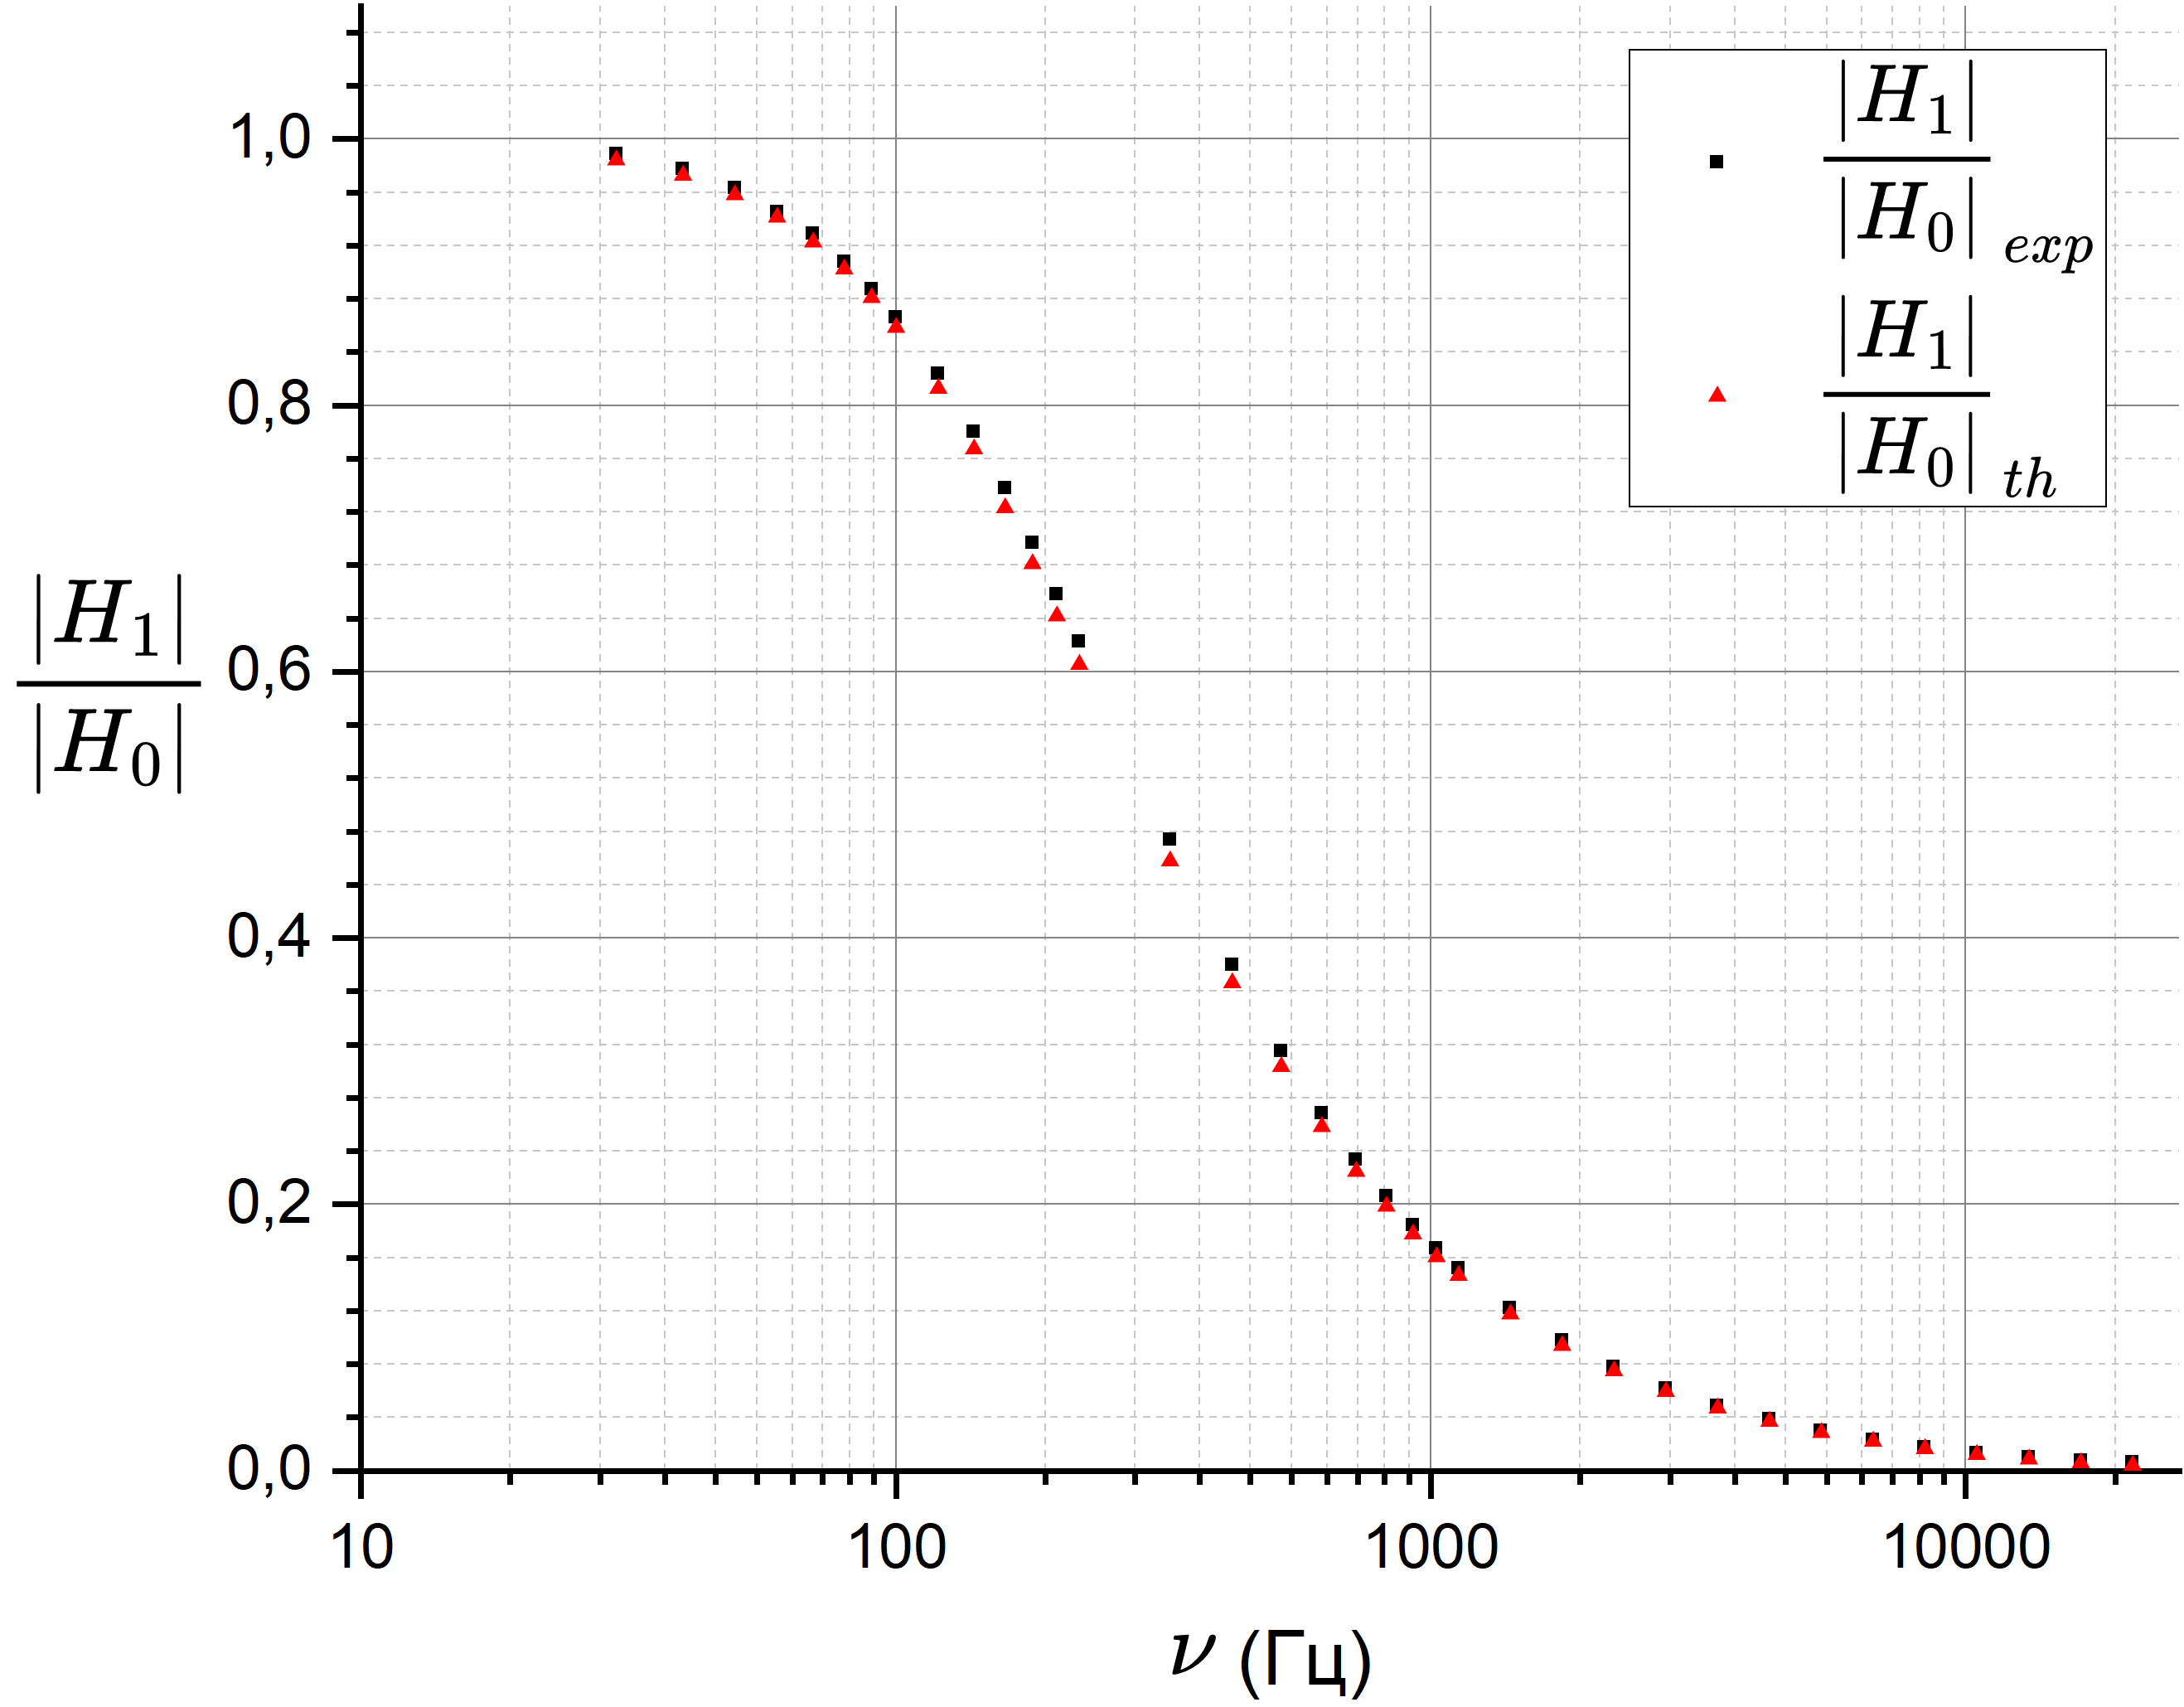
\includegraphics[width=\textwidth]{Final}
		\caption{График зависимость $\frac{|H_1|}{|H_0|}(\nu)$}
	\end{figure}
	
	\section*{Выводы}
	В данной лабораторной работе мы измеряли удельную проводимость меди 4-мя различными способами с помощью явления скин-эффекта. Запишем результаты в общую таблицу:
	
	\begin{table}[!h]
		\begin{center}
			\begin{tabular}{|l|c|c|c|}
				\hline
				Метод измерения & $\sigma, 10^{7} \ \frac{\text{См}}{\text{м}}$ & $\Delta\sigma, 10^{7} \ \frac{\text{См}}{\text{м}}$ & $\varepsilon_{\sigma}$\\
				\hline
				Отношение амплитуд & 4.294 & 0.005 & 0.1\%\\ \hline
				Разности фаз (низкие частоты) & 3.93 & 0.73 & 18.6\%\\ \hline
				Разности фаз (высокие частоты) & 3.80 & 0.58 & 15.2\%\\ \hline
				Индуктивность & 4.11 & 0.07 & 1.8\%\\ \hline
				
			\end{tabular}
		\end{center}
		\caption{Сравнение результатов различных методов}\label{}
	\end{table}
	
	В работе использовалась медь марки $M3$, для которой $\sigma_{\text{табл}} = 5.62\cdot10^{7} \ \frac{\text{См}}{\text{м}}$.
	Полученные нами значения совпадают по порядку, но, все же, немного нижу табличного значения. Несовпадение может быть вызвано многими факторами, например наводкой поля в соединительных проводах и пренебрежением размерами медного цилиндра и соленоида. 
	
	Методы измерения через разность фаз дали высокие погрешности, потому что измерения делались на глаз на осциллографе, и гарантировать их точность можно только с введенной погрешностью. Кроме того, при измерении на высоких частотах зависимость не является везде линейной, это тоже привносит свою неточность.
	
	Что касается зависимости $\frac{|H_1|}{|H_0|}(\nu)$, то экспериментальные данные очень хорошо согласуются с теоретической зависимостью.
\end{document}